\section{Asymmetric Numeral System}

\subsection{Basic Idea}
    \subsubsection{Motivation}
    \begin{frame}[fragile]{Motivation}
        ANS combines the compression ratio of \href{https://en.wikipedia.org/wiki/Arithmetic_coding}{arithmetic coding} (which uses a nearly accurate \href{https://en.wikipedia.org/wiki/Probability_distribution}{probability distribution}), with a processing cost similar to that of \href{https://en.wikipedia.org/wiki/Huffman_coding}{Huffman coding} [3]
    \end{frame}

    \begin{frame}[fragile]{Basic Idea}
        \begin{itemize}
            \item<1-> Symbol spread function
            \item<2-> Representation of information \\
            (represents an entire message as a single number, similar to Arithmetic Coding) --> example: representation of \{2,0,2,5,1,8\}
            \item<3-> Symmetric or Asymmetric
            \item<4-> rANS and tANS
        \end{itemize}
    \end{frame}

    \subsubsection{Symbol spread function}
    \begin{frame}[fragile]{Symbol spread function}
        \begin{itemize}
            \item<1-> the function that determines the split of the $\mathbb{N}$ subsets corresponding to different symbols [1]
            \item<2-> $\bar{s}: \mathbb{N} \rightarrow \mathcal{A}, \bar{s}(x) = \text{mod}(x,b) = s$
            \item<3-> In the standard binary system example: $\bar{s}(x) = \text{mod}(x,2)$ \\ e.g. splits natural numbers into subsets of even/odd numbers [1]
        \end{itemize}
    \end{frame}

    \begin{frame}[fragile]{Symbol spread function (Exa. 1)}
        $S=\{0,1\}$
        \begin{center}
            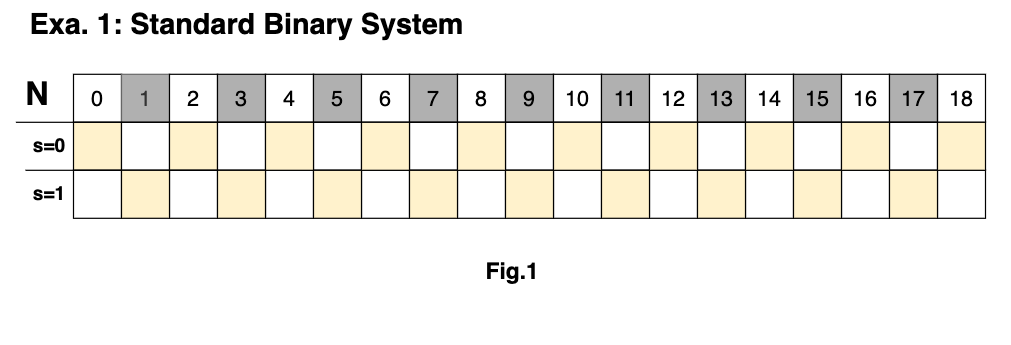
\includegraphics[width=0.9\textwidth]{../24ws_ANS.assets/exa1_1.png}
        \end{center}
    \end{frame}

    \begin{frame}[fragile]{Symbol spread function (Exa. 2)}
        $S=\{0,1,2,3,4,5,6,7,8,9\}$
        \begin{center}
            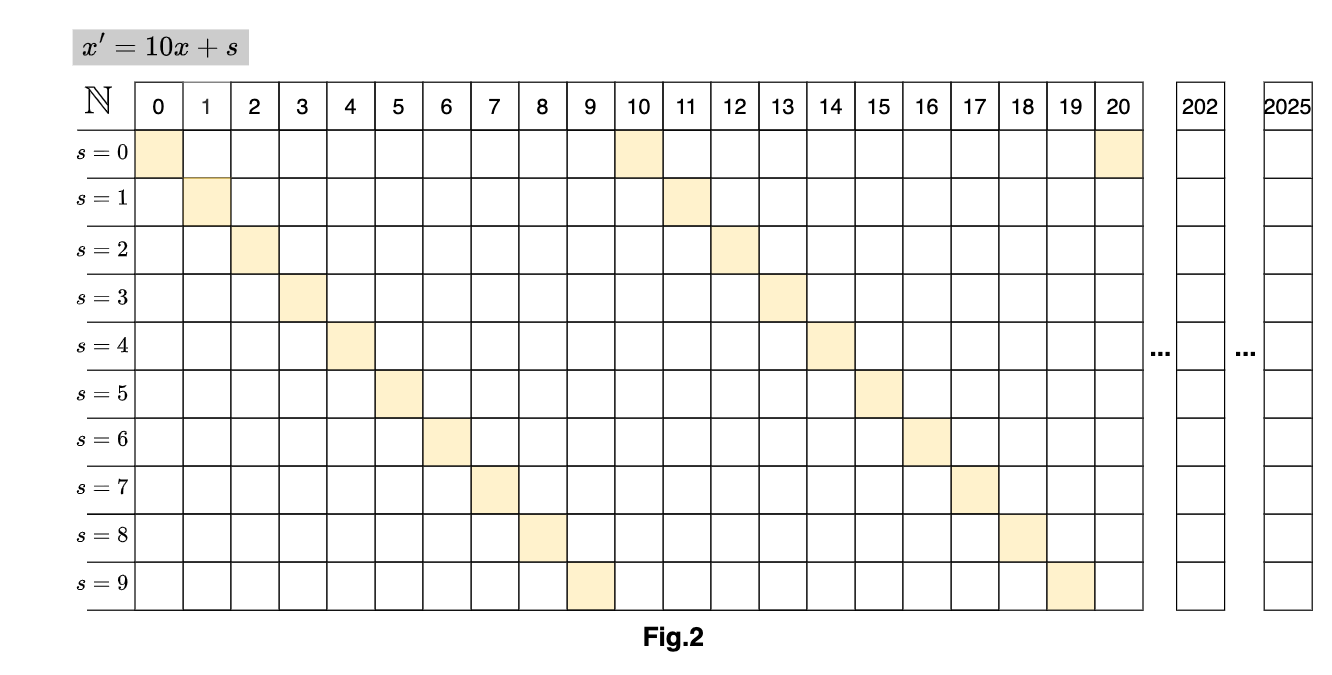
\includegraphics[width=0.85\textwidth]{../24ws_ANS.assets/fig2.png}
        \end{center}
    \end{frame}

    \subsubsection{Representation of information}    
    \begin{frame}[fragile]{Representation of information (Exa. 2)}
        \begin{itemize}
            \item<1-> a finite sequence of symbols/digits: $$\mathcal{A}=\{0,1,2,3,4,5,6,7,8,9\}$$
            \item<2-> the sequence of symbols/digits to be encoded: $$S_{in}=(2,0,2,5)$$
            \item<3-> \textcolor{red}{How can we represent this sequence as a single number?} 
            \item<4-> The easiest way is to concatenate the symbols/digits: $$x_{out} = 2025$$
        \end{itemize}
    \end{frame}

    \begin{frame}[fragile]{Representation of Information (Exa. 2)}
        \begin{itemize}
            \item<1-> encoding the sequence of digits (2,0,2,5,1,8)
            \[
            \begin{aligned}
                x_{\text{init}} &= 0 \\
                x_1 &= x_{\text{init}} \times 10 + 2 = 2 \\
                x_2 &= x_1 \times 10 + 0 = 20 \\
                x_3 &= x_2 \times 10 + 2 = 202 \\
                x_{\text{out}} &= x_3 \times 10 + 5 = 2025
            \end{aligned}
            \]
        \end{itemize}
    \end{frame}

    \begin{frame}[fragile]{Representation of Information (Exa. 2)}
        \begin{itemize}
            \item<1-> \textcolor{red}{What is the encoding function?}
            \item<2-> Encoding function
            $$x_{i+1} = x_i \times 10 + s_i$$
            \item<3-> x' is the x-th appearance of symbol s
            $$x' = \textcolor{orange}{C(s, x)= x \cdot 10 + s} $$
        \end{itemize}
    \end{frame}

    \begin{frame}[fragile]{Representation of Information (Exa. 2)}
        \begin{center}
            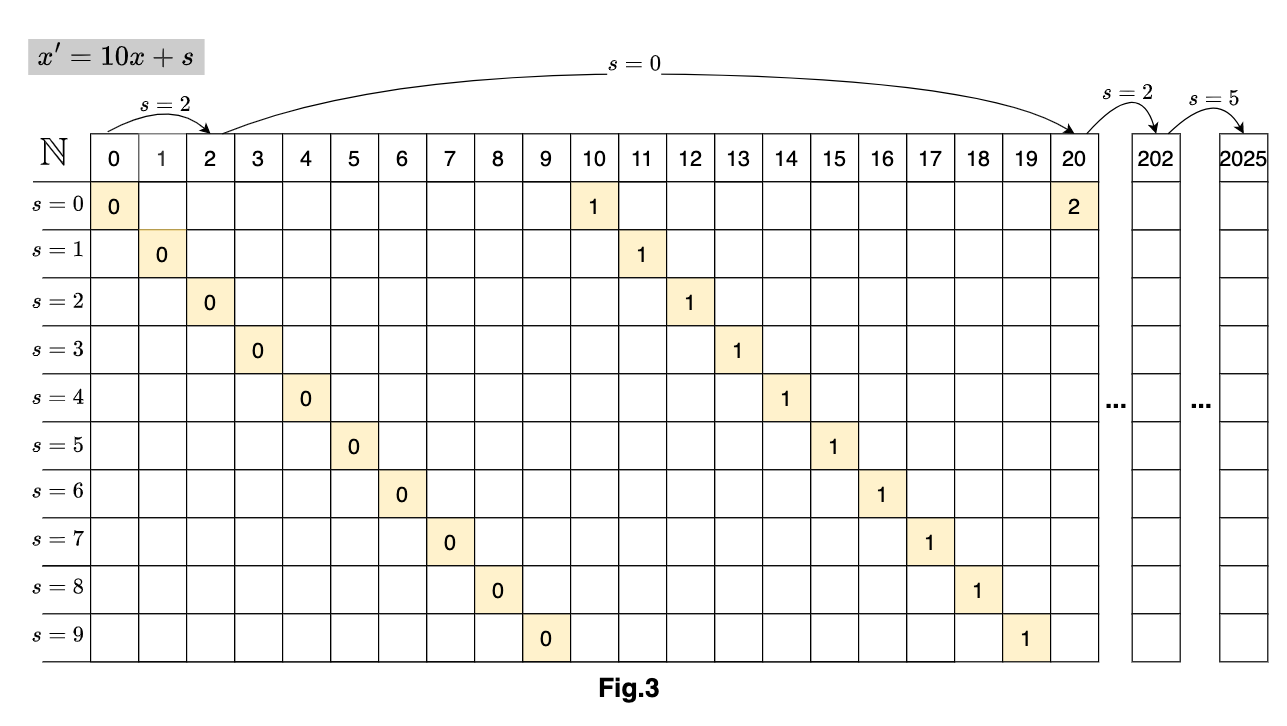
\includegraphics[width=0.85\textwidth]{../24ws_ANS.assets/fig3.png}    
        \end{center}
    \end{frame}

    \begin{frame}[fragile]{Representation of Information (Exa. 1)}
        \begin{center}
            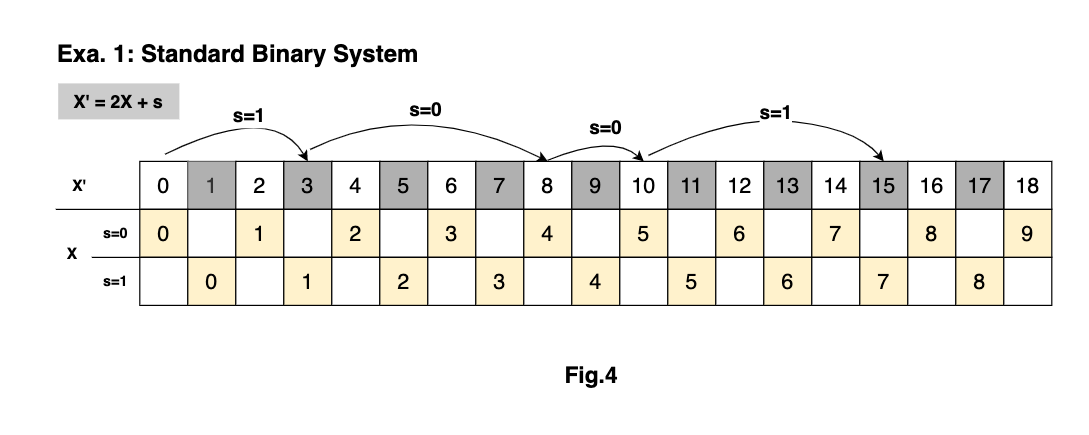
\includegraphics[width=0.95\textwidth]{../24ws_ANS.assets/fig4.png}    
        \end{center}
    \end{frame}

    \begin{frame}[fragile]{}
        \begin{center}
            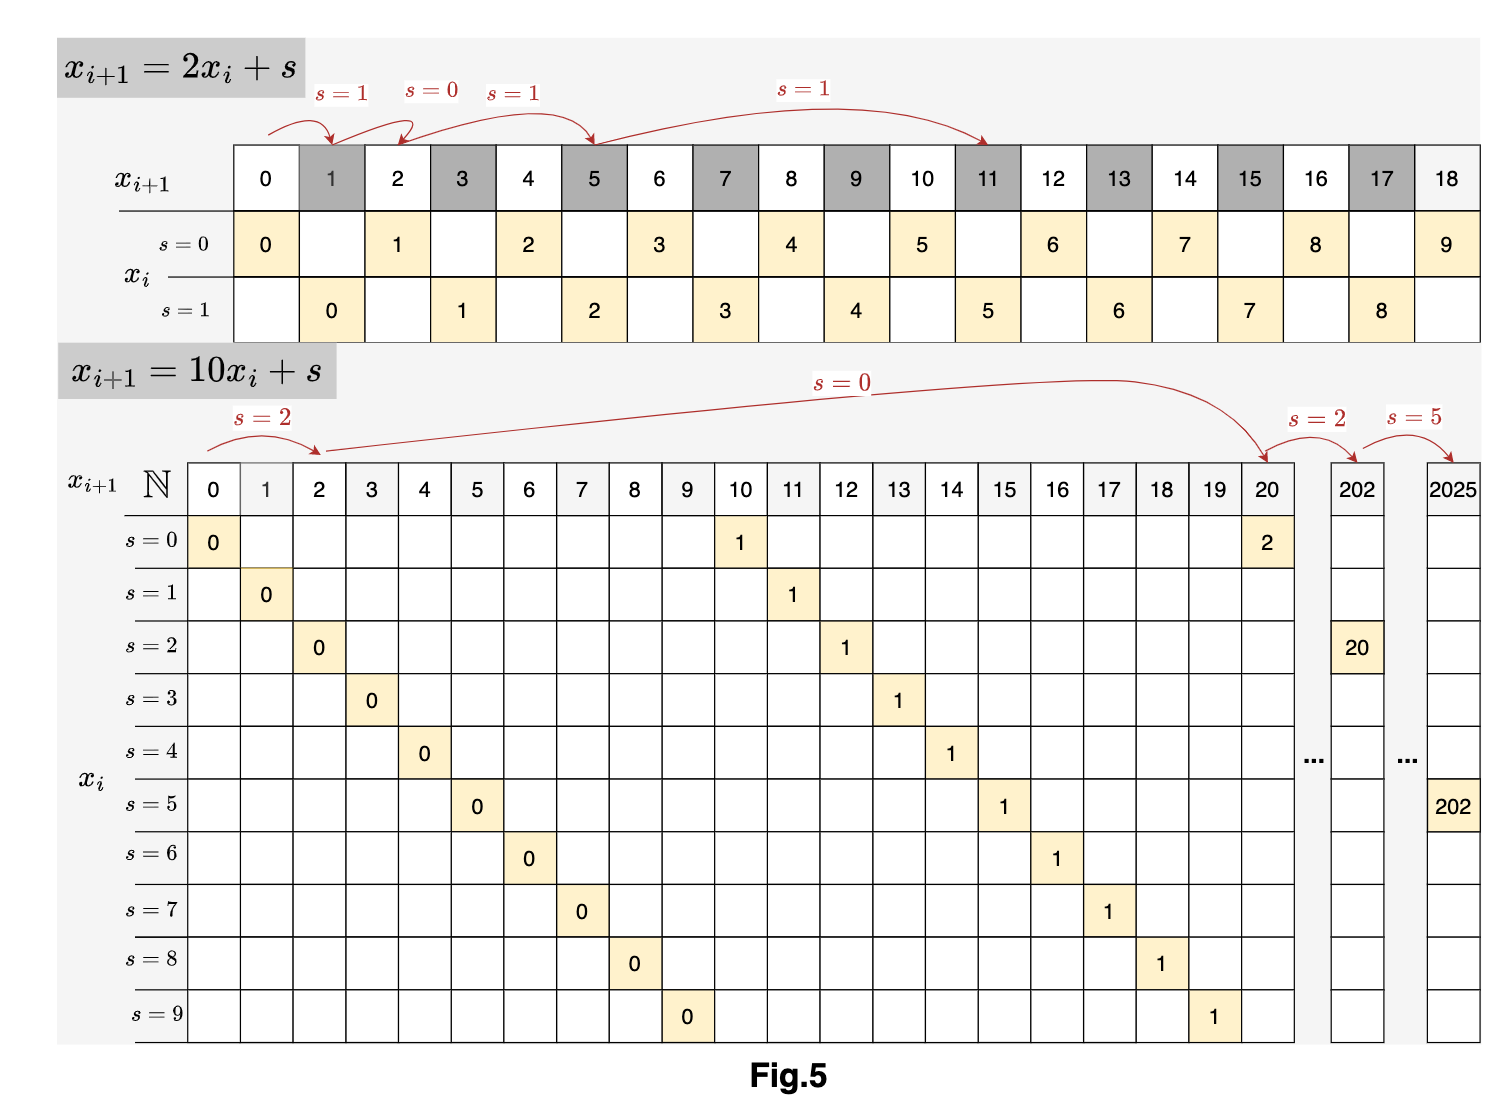
\includegraphics[width=0.7\textwidth]{../24ws_ANS.assets/fig5.png}  
        \end{center}
    \end{frame}

    \subsubsection{Symmetric or Asymmetric}
    \begin{frame}[fragile]{}
        \begin{center}
            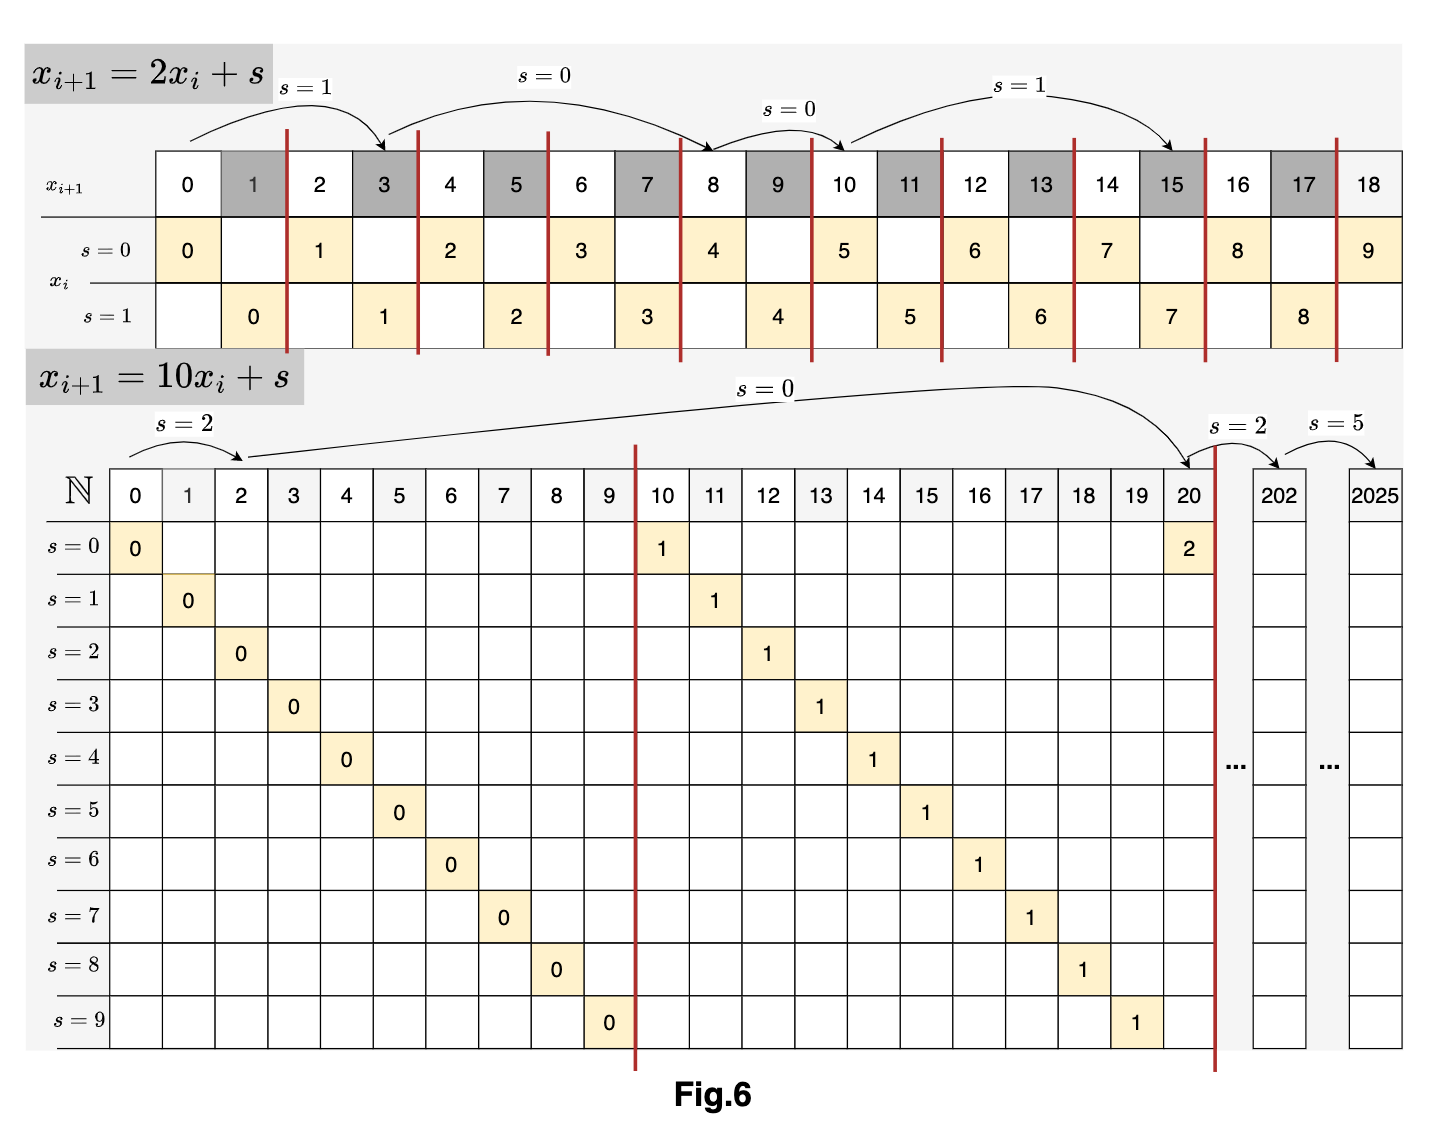
\includegraphics[width=0.7\textwidth]{../24ws_ANS.assets/fig6.png}  
        \end{center}
    \end{frame}

    \begin{frame}[fragile]{Exa. 3: Asymmetric Binary System}
        \begin{itemize}
            \item<1-> Let $\mathcal{A} = \{0,1\}$
            \item<1-> $Pr(0) = 1/4, Pr(1)= 3/4$ 
            \item<2-> a cycle of length 4, which contains 1 zero and 3 ones
            \item<3-> $x' = C(s,x) \approx x/p_s$
            % \item $C(0,x)=4x$, $C(1,x)=4\lfloor x/3 \rfloor + mod(x,3) + 1$
        \end{itemize}
    \end{frame}

    \begin{frame}[fragile]{Exa. 3: Asymmetric Binary System}
        \begin{center}
            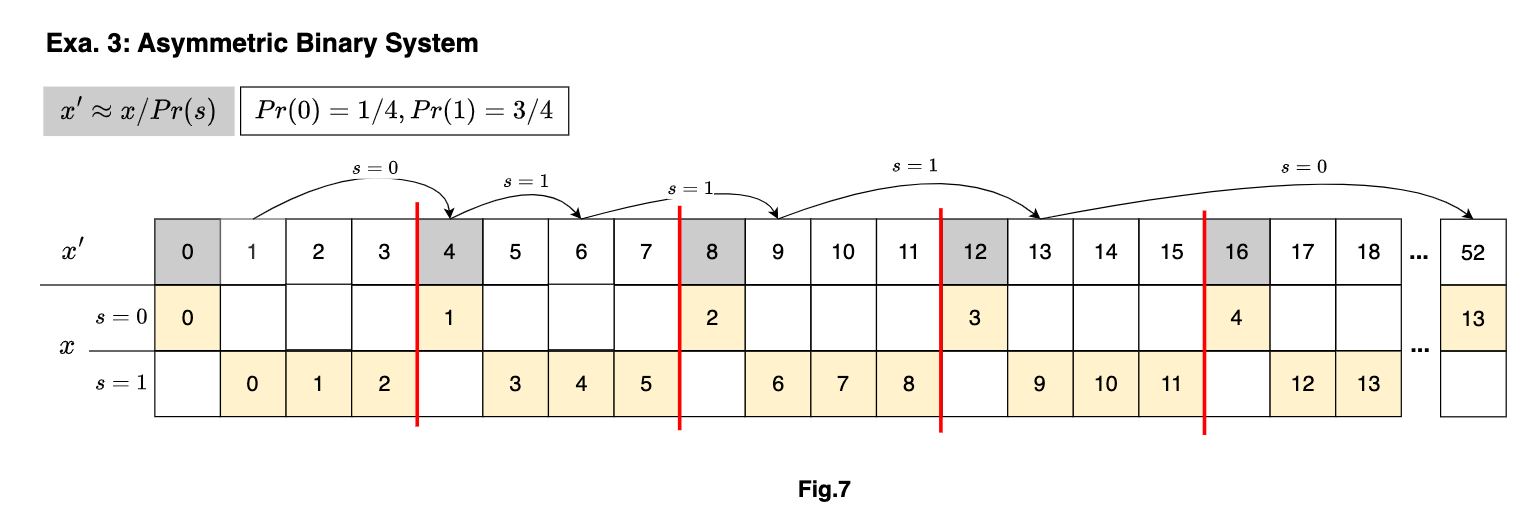
\includegraphics[width=0.9\textwidth]{../24ws_ANS.assets/fig7.png}
        \end{center}
        We refine even/odd number by changing their densities
    \end{frame}

    \begin{frame}[fragile]{Symmetric or Asymmetric}
        \begin{itemize}
            \item Symmetric: uniform distribution
            \item Asymmetric: non-uniform distribution
        \end{itemize}
    \end{frame}

\subsection{rANS}
    \subsubsection{Key Concepts}
    \begin{frame}[fragile]{rANS}
        \begin{itemize}
            \item "r" = "range": similar to range coding (RC)
            \item symbol spread function
            \item representation of information
            \item asymmetric
        \end{itemize}
    \end{frame}

    \subsubsection{Exa. 3}
    \begin{frame}[fragile]{Exa.3}
        How to encode 101110? What is the encoding function $C(s,x)$? \ $x' = C(s,x) \approx x/p_s$
    \end{frame}
    \begin{frame}[plain]
        \begin{figure}
            \centering
            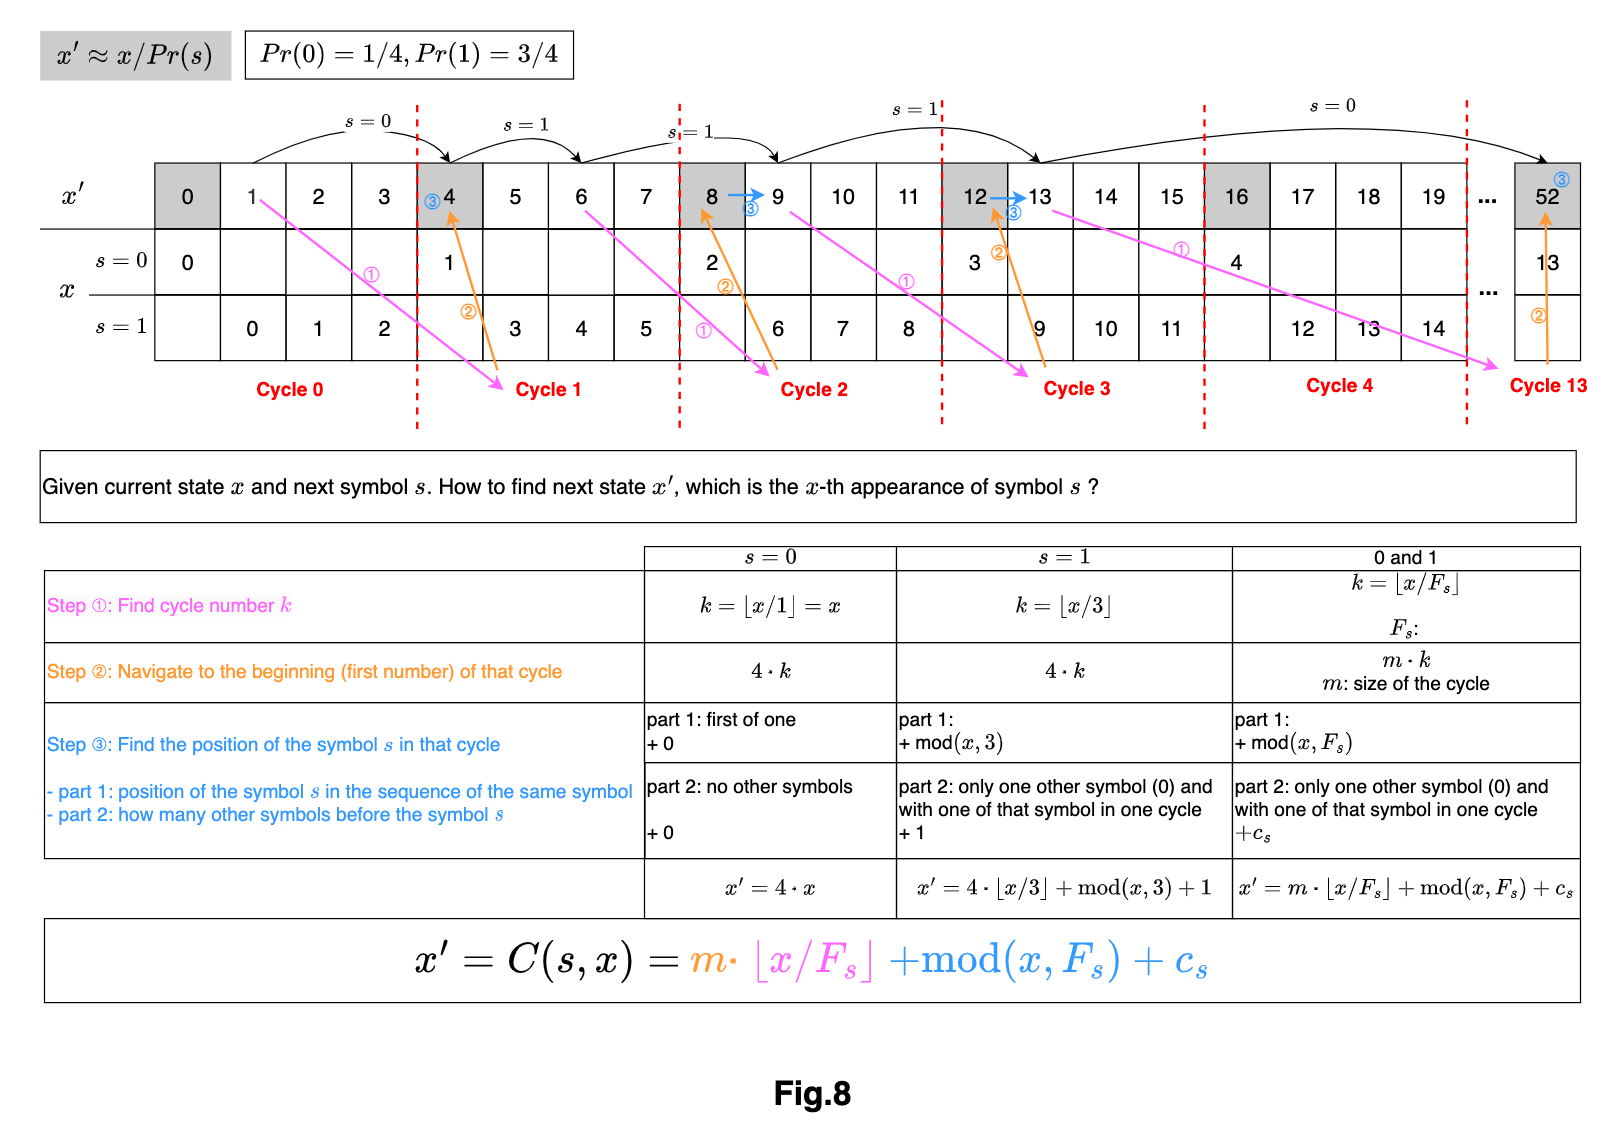
\includegraphics[width=1\textwidth,height=1.07\textheight,keepaspectratio]{../24ws_ANS.assets/fig8.png}
        \end{figure}
    \end{frame}

    \subsubsection{Encoding Function}
    \begin{frame}[fragile]{}
        \textbf{Encoding Function (general):}
        \[
        x' = m \cdot \left\lfloor \frac{x}{F_s} \right\rfloor + \operatorname{mod}(x, F_s) + c_s
        \]
        \begin{itemize}
            \item \textbf{Alphabet set:} \(\mathcal{A} = \{a_1, a_2, \dots, a_k\}\)
            \item \textbf{Absolute frequency of symbol \(s\):} \(F_s\)
            \item \textbf{Total frequency:} $m = \sum_{i=1}^{k} F_i$
            \item \textbf{Probability of symbol \(s\):} $p_s = \frac{F_s}{m}$
            \item \textbf{Cumulative frequency before \(s\):} $c_s := F_0 + F_1 + \dots + F_{s-1}$
            % \item \textbf{Input sequence:} 
            % \[
            % S_{\text{in}} = (s_1, s_2, \dots, s_n)
            % \]
        \end{itemize}
    \end{frame}

    \begin{frame}[fragile]{}
        \textbf{Encoding Function (binary):}
        \[
        x' = C(s,x) = \left\lfloor \frac{x}{F_s} \right\rfloor << n+ \operatorname{mod}(x, F_s) + c_s \, ^{[1]}
        \]
        \begin{itemize}
            \item \textbf{Alphabet set:} \(\mathcal{A} = \{a_1, a_2, \dots, a_k\}\)
            \item \textbf{Absolute frequency of symbol \(s\):} \(F_s\)
            \item \textbf{Total frequency:} $m = \sum_{i=1}^{k} F_i$
            \item \textbf{Probability of symbol \(s\):} $p_s = \frac{F_s}{m}$
            \item \textbf{Cumulative frequency before \(s\):} $c_s := F_0 + F_1 + \dots + F_{s-1}$
            \item $<< n$ is a left shift by $n$ bits
            % \item \textbf{Input sequence:} 
            % \[
            % S_{\text{in}} = (s_1, s_2, \dots, s_n)
            % \]
        \end{itemize}
    \end{frame}

    \subsubsection{Decoding Function}
    \begin{frame}
        \textbf{Decoding Function (binary):}
        \[
        D(x) = (s, F_s \cdot (x >> n)+ (x \& mask) - c_s) ^{[1]}
        \]
        \begin{itemize}
            \item 
        \end{itemize}
    \end{frame}
    \subsubsection{Streaming-rANS}
    \begin{frame}[fragile]{Streaming-rANS}
        To avoid using large number arithmetic, in practice stream variants are used: which enforce by renormalization: sending the least significant bits of x to or from the bitstream (usually L and b are powers of 2).
    \end{frame}


\subsection{tANS}
    \begin{frame}[fragile]{tANS}
        \begin{itemize}
            \item d
        \end{itemize}
    \end{frame}

\subsection{Performance}
\begin{frame}[fragile]{Performance}
    \begin{itemize}
        \item f
    \end{itemize}
\end{frame}
